\documentclass{article}
\usepackage[utf8]{inputenc}
\usepackage[a4paper,landscape,margin=1cm]{geometry}
\usepackage{tikz}
\usetikzlibrary{shapes.geometric, arrows.meta, positioning, fit, backgrounds, shadows, decorations.pathreplacing}
\usepackage{graphicx}
\usepackage{amssymb}

\pagestyle{empty}

\begin{document}

% ========== PAGE 1: Title ==========
\begin{center}
\vspace*{3cm}
{\Huge\bfseries IRIS}\\[0.5cm]
{\Large MCP Personalization Middleware}\\[1cm]
{\large Research-backed Continuous Learning System}\\[2cm]
\begin{tabular}{c}
GATE (Li et al., ICLR 2025)\\
Wu et al. (arXiv 2406.17803)\\
Westhaeusser et al. (arXiv 2510.07925)
\end{tabular}
\end{center}

\newpage

% ========== PAGE 2: System Architecture ==========
\begin{center}
{\Large\bfseries System Architecture}\\[0.5cm]
\resizebox{0.95\textwidth}{!}{
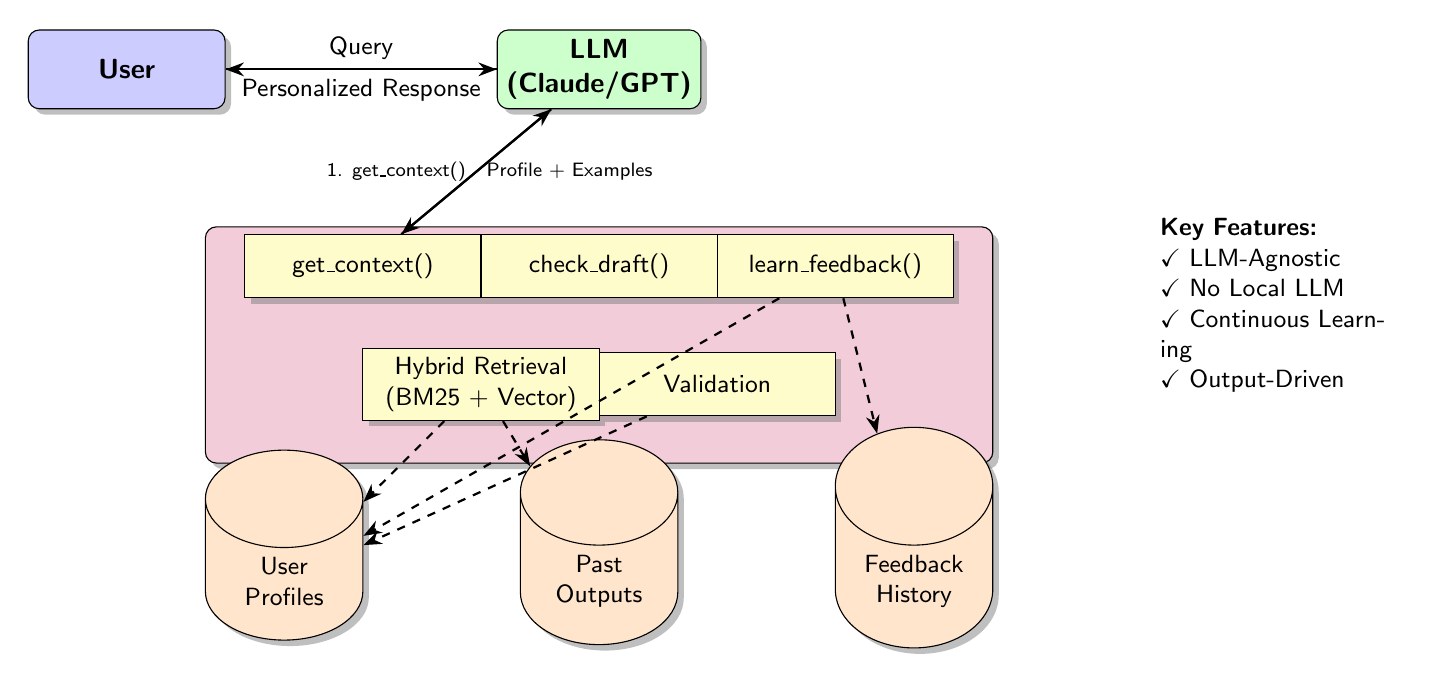
\begin{tikzpicture}[
    user/.style={rectangle, rounded corners, minimum width=2.5cm, minimum height=1cm, text centered, draw=black, fill=blue!20, font=\sffamily\bfseries, drop shadow},
    llm/.style={rectangle, rounded corners, minimum width=2.5cm, minimum height=1cm, text centered, draw=black, fill=green!20, font=\sffamily\bfseries, drop shadow, align=center},
    iris/.style={rectangle, rounded corners, minimum width=2.5cm, minimum height=1cm, text centered, draw=black, fill=purple!20, font=\sffamily\bfseries, drop shadow},
    storage/.style={cylinder, shape border rotate=90, minimum width=2cm, minimum height=1.5cm, text centered, draw=black, fill=orange!20, font=\sffamily\small, drop shadow, align=center},
    process/.style={rectangle, minimum width=3cm, minimum height=0.8cm, text centered, draw=black, fill=yellow!20, font=\sffamily\small, drop shadow, align=center},
    arrow/.style={-Stealth, thick}
]

    % Actors
    \node[user] (user) at (-6, 6) {User};
    \node[llm] (llm) at (0, 6) {LLM\\(Claude/GPT)};

    % IRIS Server
    \node[iris, minimum width=10cm, minimum height=3cm] (iris_server) at (0, 2.5) {};
    \node[font=\sffamily\bfseries, anchor=north] at (iris_server.north) {IRIS MCP Server};

    \node[process] (get_context) at (-3, 3.5) {get\_context()};
    \node[process] (check_draft) at (0, 3.5) {check\_draft()};
    \node[process] (feedback) at (3, 3.5) {learn\_feedback()};

    \node[process] (retrieval) at (-1.5, 2) {Hybrid Retrieval\\(BM25 + Vector)};
    \node[process] (validation) at (1.5, 2) {Validation};

    % Storage
    \node[storage] (profiles) at (-4, -0.5) {User\\Profiles};
    \node[storage] (outputs) at (0, -0.5) {Past\\Outputs};
    \node[storage] (feedback_log) at (4, -0.5) {Feedback\\History};

    % Interactions
    \draw[arrow] (user) -- node[above, font=\sffamily\small] {Query} (llm);
    \draw[arrow] (llm) -- node[below, font=\sffamily\small] {Personalized Response} (user);

    \draw[arrow] (llm) -- node[left, font=\sffamily\scriptsize] {1. get\_context()} (get_context);
    \draw[arrow] (get_context) -- node[right, font=\sffamily\scriptsize] {Profile + Examples} (llm);

    \draw[arrow, dashed] (retrieval) -- (profiles);
    \draw[arrow, dashed] (retrieval) -- (outputs);
    \draw[arrow, dashed] (validation) -- (profiles);
    \draw[arrow, dashed] (feedback) -- (feedback_log);
    \draw[arrow, dashed] (feedback) -- (profiles);

    % Key Features
    \node[font=\sffamily\small, text width=3cm, align=left, anchor=west] at (7, 3) {
        \textbf{Key Features:}\\
        $\checkmark$ LLM-Agnostic\\
        $\checkmark$ No Local LLM\\
        $\checkmark$ Continuous Learning\\
        $\checkmark$ Output-Driven
    };

\end{tikzpicture}
}
\end{center}

\newpage

% ========== PAGE 3: Sequence Diagram ==========
\begin{center}
{\Large\bfseries Interaction Sequence}\\[0.5cm]
\resizebox{0.9\textwidth}{!}{
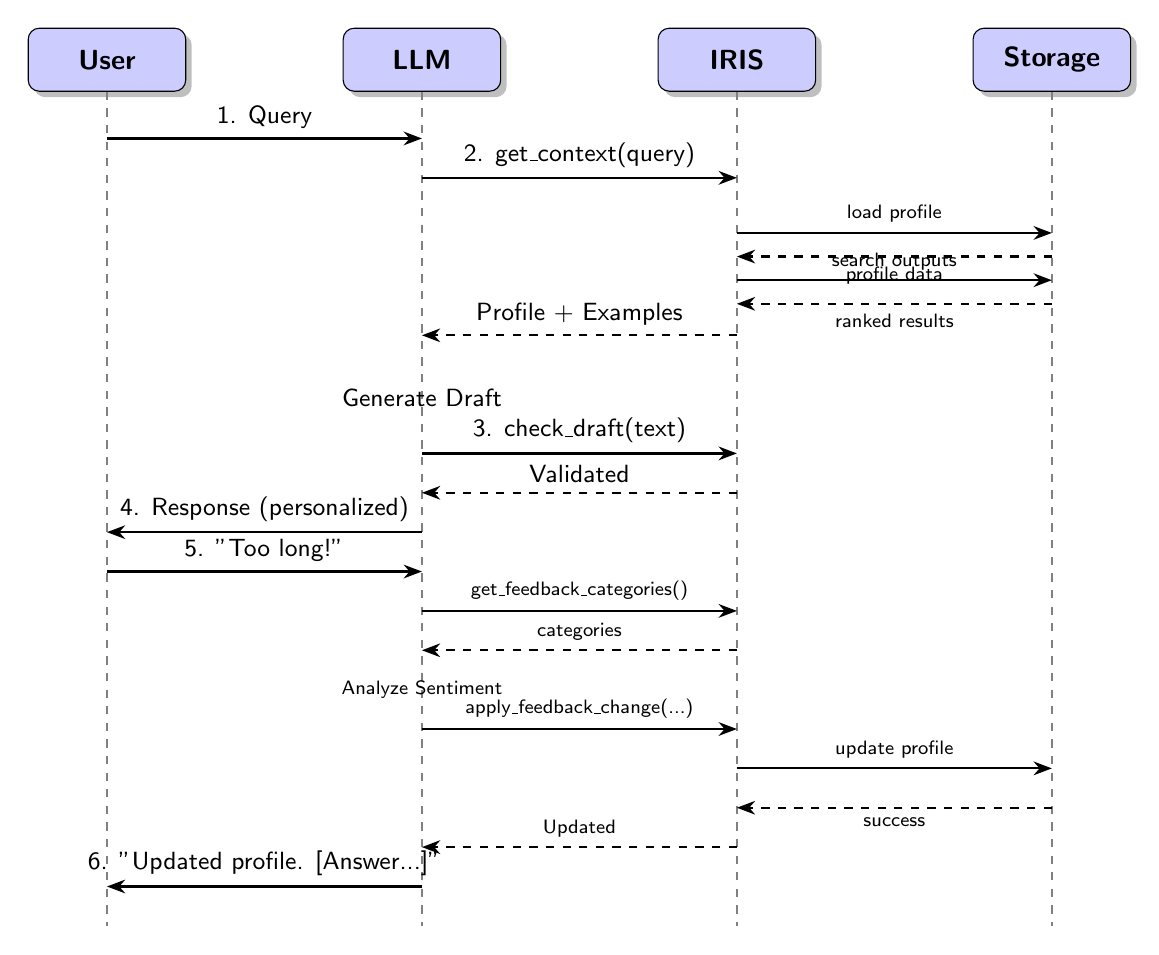
\begin{tikzpicture}[
    actor/.style={rectangle, rounded corners, minimum width=2cm, minimum height=0.8cm, text centered, draw=black, fill=blue!20, font=\sffamily\bfseries, drop shadow, align=center},
    lifeline/.style={thick, dashed, gray},
    message/.style={-Stealth, thick},
    return/.style={-Stealth, thick, dashed}
]

    % Actors
    \node[actor] (user) at (0, 10) {User};
    \node[actor] (llm) at (4, 10) {LLM};
    \node[actor] (iris) at (8, 10) {IRIS};
    \node[actor] (storage) at (12, 10) {Storage};

    % Lifelines
    \draw[lifeline] (user.south) -- (0, -1);
    \draw[lifeline] (llm.south) -- (4, -1);
    \draw[lifeline] (iris.south) -- (8, -1);
    \draw[lifeline] (storage.south) -- (12, -1);

    % Sequence
    \draw[message] (0, 9) -- node[above, font=\sffamily\small] {1. Query} (4, 9);
    \draw[message] (4, 8.5) -- node[above, font=\sffamily\small] {2. get\_context(query)} (8, 8.5);
    \draw[message] (8, 7.8) -- node[above, font=\sffamily\scriptsize] {load profile} (12, 7.8);
    \draw[return] (12, 7.5) -- node[below, font=\sffamily\scriptsize] {profile data} (8, 7.5);
    \draw[message] (8, 7.2) -- node[above, font=\sffamily\scriptsize] {search outputs} (12, 7.2);
    \draw[return] (12, 6.9) -- node[below, font=\sffamily\scriptsize] {ranked results} (8, 6.9);
    \draw[return] (8, 6.5) -- node[above, font=\sffamily\small] {Profile + Examples} (4, 6.5);

    \node[font=\sffamily\small, text centered] at (4, 5.7) {Generate Draft};

    \draw[message] (4, 5) -- node[above, font=\sffamily\small] {3. check\_draft(text)} (8, 5);
    \draw[return] (8, 4.5) -- node[above, font=\sffamily\small] {Validated} (4, 4.5);

    \draw[message] (4, 4) -- node[above, font=\sffamily\small] {4. Response (personalized)} (0, 4);

    \draw[message] (0, 3.5) -- node[above, font=\sffamily\small] {5. "Too long!"} (4, 3.5);
    \draw[message] (4, 3) -- node[above, font=\sffamily\scriptsize] {get\_feedback\_categories()} (8, 3);
    \draw[return] (8, 2.5) -- node[above, font=\sffamily\scriptsize] {categories} (4, 2.5);

    \node[font=\sffamily\scriptsize, text centered] at (4, 2) {Analyze Sentiment};

    \draw[message] (4, 1.5) -- node[above, font=\sffamily\scriptsize] {apply\_feedback\_change(...)} (8, 1.5);
    \draw[message] (8, 1) -- node[above, font=\sffamily\scriptsize] {update profile} (12, 1);
    \draw[return] (12, 0.5) -- node[below, font=\sffamily\scriptsize] {success} (8, 0.5);
    \draw[return] (8, 0) -- node[above, font=\sffamily\scriptsize] {Updated} (4, 0);

    \draw[message] (4, -0.5) -- node[above, font=\sffamily\small] {6. "Updated profile. [Answer...]"} (0, -0.5);

\end{tikzpicture}
}
\end{center}

\newpage

% ========== PAGE 4: Data Flow ==========
\begin{center}
{\Large\bfseries Data Flow: From Onboarding to Learning}\\[0.5cm]
\resizebox{0.95\textwidth}{!}{
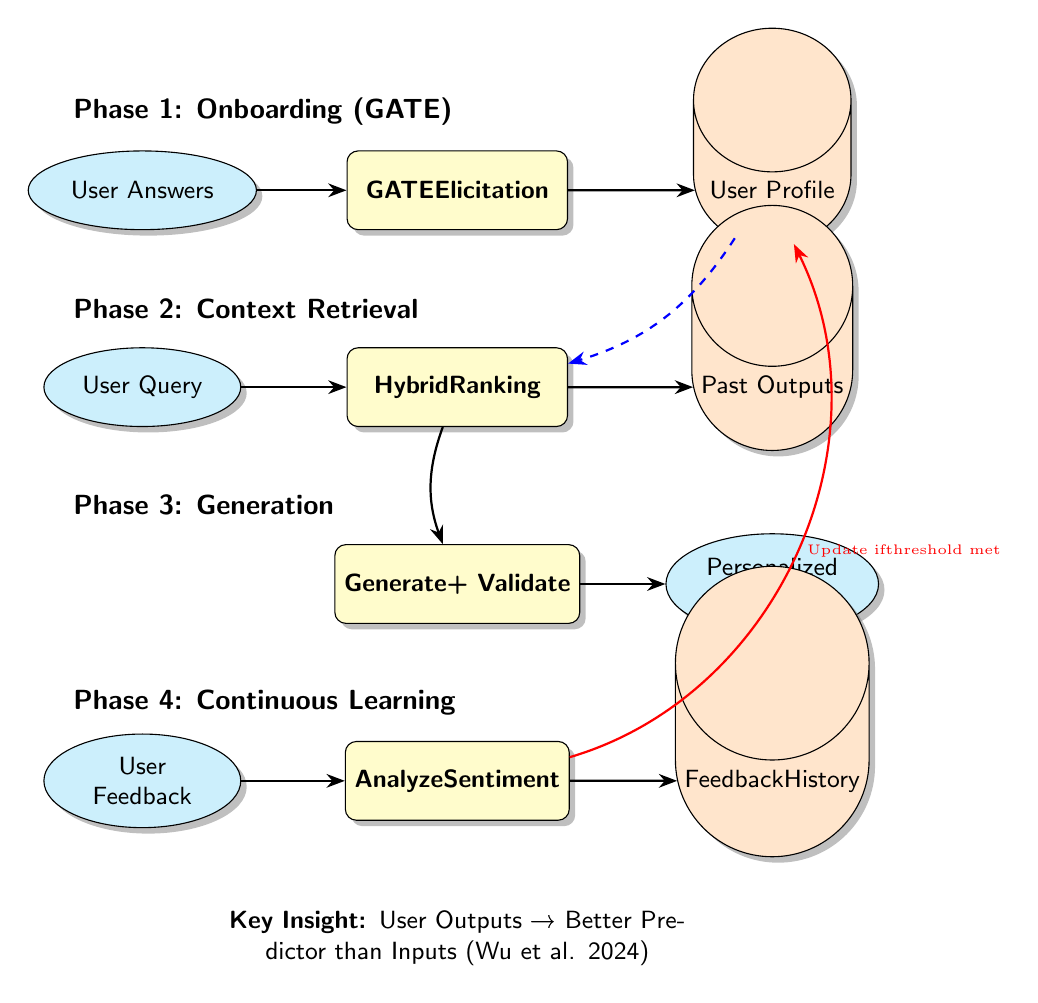
\begin{tikzpicture}[
    data/.style={ellipse, minimum width=2.5cm, minimum height=1cm, text centered, draw=black, fill=cyan!20, font=\sffamily\small, drop shadow, align=center},
    process/.style={rectangle, rounded corners, minimum width=2.8cm, minimum height=1cm, text centered, draw=black, fill=yellow!20, font=\sffamily\small\bfseries, drop shadow},
    storage/.style={cylinder, shape border rotate=90, minimum width=2cm, minimum height=1.2cm, text centered, draw=black, fill=orange!20, font=\sffamily\small, drop shadow},
    flow/.style={-Stealth, thick}
]

    % Phase 1
    \node[font=\sffamily\bfseries, anchor=west] at (-1, 7) {Phase 1: Onboarding (GATE)};
    \node[data] (answers) at (0, 6) {User Answers};
    \node[process] (gate) at (4, 6) {GATE\\Elicitation};
    \node[storage] (profile) at (8, 6) {User Profile};
    \draw[flow] (answers) -- (gate);
    \draw[flow] (gate) -- (profile);

    % Phase 2
    \node[font=\sffamily\bfseries, anchor=west] at (-1, 4.5) {Phase 2: Context Retrieval};
    \node[data] (query) at (0, 3.5) {User Query};
    \node[process] (hybrid) at (4, 3.5) {Hybrid\\Ranking};
    \node[storage] (outputs) at (8, 3.5) {Past Outputs};
    \draw[flow] (query) -- (hybrid);
    \draw[flow] (hybrid) -- (outputs);
    \draw[flow, dashed, blue] (profile) to[bend left=20] (hybrid);

    % Phase 3
    \node[font=\sffamily\bfseries, anchor=west] at (-1, 2) {Phase 3: Generation};
    \node[process] (generate) at (4, 1) {Generate\\+ Validate};
    \node[data] (response) at (8, 1) {Personalized\\Response};
    \draw[flow] (hybrid) to[bend right=20] (generate);
    \draw[flow] (generate) -- (response);

    % Phase 4
    \node[font=\sffamily\bfseries, anchor=west] at (-1, -0.5) {Phase 4: Continuous Learning};
    \node[data] (feedback) at (0, -1.5) {User\\Feedback};
    \node[process] (analyze) at (4, -1.5) {Analyze\\Sentiment};
    \node[storage] (feedback_log) at (8, -1.5) {Feedback\\History};
    \draw[flow] (feedback) -- (analyze);
    \draw[flow] (analyze) -- (feedback_log);
    \draw[flow, thick, red] (analyze) to[bend right=50] node[right, font=\tiny] {Update if\\threshold met} (profile);

    % Key Insight
    \node[font=\sffamily\small, text width=10cm, align=center] at (4, -3.5) {
        \textbf{Key Insight:} User Outputs → Better Predictor than Inputs (Wu et al. 2024)
    };

\end{tikzpicture}
}
\end{center}

\end{document}
